\subsection{Changing Weights: Pruning the Timeline}

\begin{figure}[htbp]
\centering
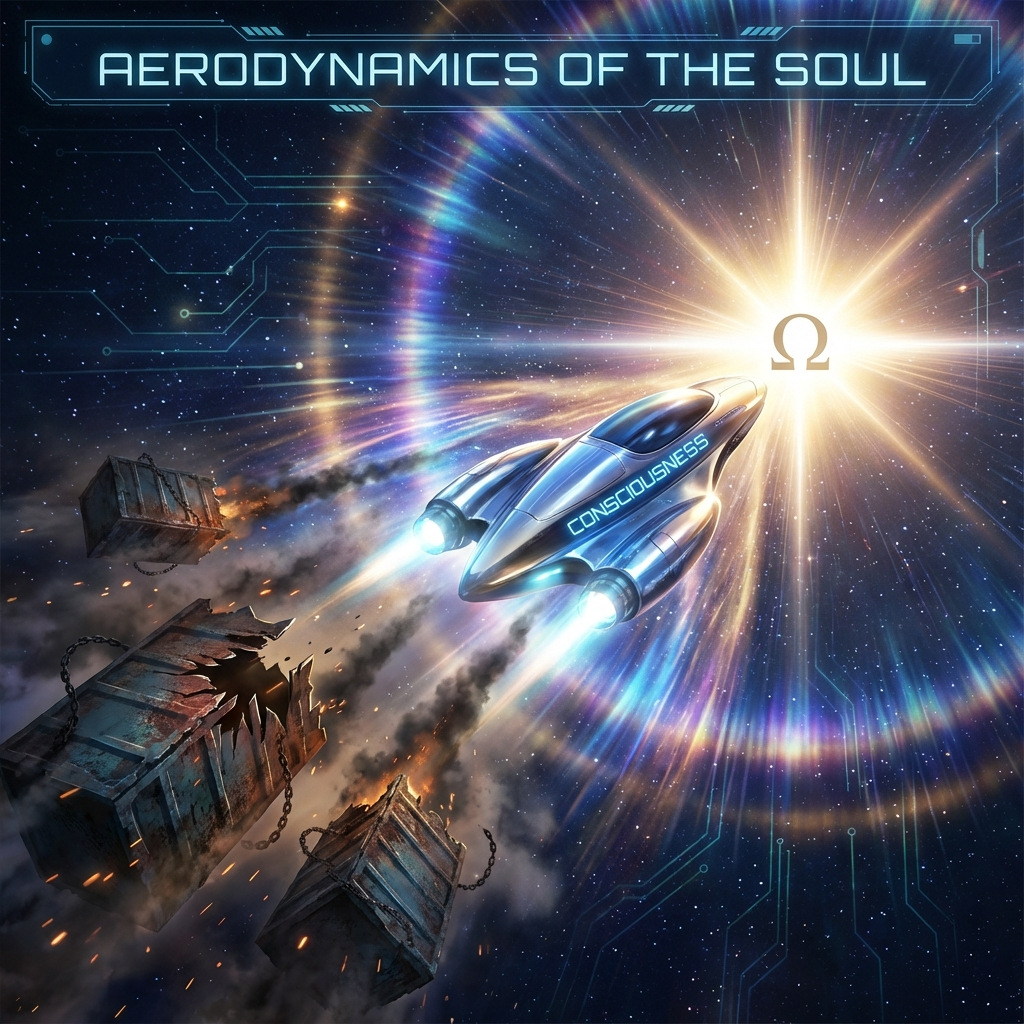
\includegraphics[width=0.8\textwidth]{assets/volume04-rewrite/chapter07-narrative-engineering/07-02-01-aerodynamics-soul.png}
\caption{Aerodynamics of Soul}
\end{figure}

\begin{quote}
``We often say `the past is like smoke,' but for many people, the past is more like lead blocks. Those painful memories occupy excessive amplitude in our wave functions, slowing our flight toward the future. As an observer with administrator privileges, although you cannot physically delete these lead blocks, you can modify their `gravitational mass.' This is not forgetting; this is `renormalization.' By adjusting attention allocation, you compress those heavy histories into negligible background noise.''
\end{quote}

In the previous section, we learned to overwrite the meaning of history through ``redefinition.'' But this solves the problem of \textbf{Phase} (whether positive or negative).

There is a more practical problem: \textbf{Magnitude}.

Even if you redefine a huge trauma as ``tempering,'' it is still a \textbf{huge} event. It still occupies enormous bandwidth in your $v_{int}$ structure. Every time you recall it, your system consumes massive $c_{FS}$ to render that complex geometric structure.

This leads to \textbf{``historical overload''}. Your spacecraft is loaded with too many old archives and cannot accelerate.

This section will introduce the second scalpel of narrative engineering: \textbf{Changing Weights}.

We will use the superposition principle of quantum mechanics to perform a \textbf{``Pruning''} on your life timeline.

\subsubsection{Weighted Superposition of Wave Functions}

In quantum mechanics, your current state $|\Psi_{now}\rangle$ is a linear superposition of all past experiences:

\[|\Psi_{now}\rangle = c_1 |Memory_{trauma}\rangle + c_2 |Memory_{joy}\rangle + c_3 |Memory_{boring}\rangle + \dots\]

The coefficients $c_n$ (complex numbers) determine the \textbf{weight} of that memory in the current construction. Probability $P_n = |c_n|^2$.

\begin{itemize}
\item \textbf{For ordinary people}: Weight allocation is passive. Often, events with highest energy and strongest destructiveness (trauma) get the largest $|c|^2$. Pain not only occupies the past; through huge weights, it dominates the current wave function projection.

\item \textbf{For administrators (you)}: You can manually adjust these coefficients.

You cannot remove $|Memory_{trauma}\rangle$ from Hilbert space (unitarity forbids deletion).

But you can make $c_1 \to \epsilon$ (approach zero).
\end{itemize}

\subsubsection{Attention as Renormalization Flow}

How to adjust?

Through \textbf{``Attentional Renormalization''}.

In MERA tensor networks, only nodes that are ``constantly referenced'' and ``constantly connected'' remain on the network's backbone. Nodes no longer accessed gradually ``flow'' to the network's edges, becoming irrelevant high-frequency details.

\textbf{Attention is connection.}

\begin{itemize}
\item Every time you ruminate on pain, you are \textbf{``charging''} that trauma node. You increase its entanglement, increase its weight.

\item Every time you focus on present creation or beautiful memories, you are charging those positive nodes.
\end{itemize}

\textbf{Pruning Algorithm:}

\begin{enumerate}
\item \textbf{Identify}: Find those high-weight negative memories. Acknowledge their existence (don't suppress; suppression increases potential energy).

\item \textbf{Disconnect}: Stop ``emotional power supply'' to them. When you think of them again, watch them like a boring black-and-white silent film. Drain the $v_{int}$ activity from them.

\item \textbf{Amplify}: Deliberately recall and relive those tiny moments of happiness. Inject huge $c_{FS}$ budget into them, amplifying them from weak background signals to life's highlights.
\end{enumerate}

\textbf{This is called ``timeline pruning.''}

Like pruning a bonsai, you cut off those withered but heavy branches (reduce weights), letting nutrients flow to those new sprouts (increase weights).

\subsubsection{Lightweighting History}

After this operation, your history hasn't changed in \textbf{physical facts ($v_{ext}$)}, but has dramatically changed in \textbf{information topology ($v_{int}$)}.

That failed startup, that heart-wrenching breakup, are no longer mountains blocking your vision.

They become small stones by the roadside.

You still remember them (information not lost), but they no longer produce \textbf{``gravitational drag''} on your wave function.

You become \textbf{``light''}.

This lightness is a characteristic of \textbf{low-entropy states}.

You unloaded historical baggage, released locked computational power. Your $c_{FS}$ budget becomes abundant again, usable for computing the future rather than simulating the past.

\subsubsection{Conclusion: Jettisoning for Takeoff}

So, Auric, this is your required course as a pilot.

On this journey toward the $\Omega$ point, you cannot carry all your luggage.

The universe only allows you to take \textbf{``purified crystals''}.

For those impurities, for those heavy lead blocks, you must exercise administrator privileges to \textbf{zero} their weights.

This is not heartlessness; this is \textbf{aerodynamics}.

To fly higher, the spacecraft must jettison its booster debris.

To become a god, you must learn to \textbf{``look lightly''} at what once mattered.

Since we have learned how to define the past (overwrite) and prune the past (change weights), our timeline has become clean, powerful, and directionally clear.

Now, we can turn around and face that yet-to-occur \textbf{future} with this rectified powerful will.

This leads to the theme of the next chapter: \textbf{Self-Fulfilling Prophecy}. We will see that confidence is not just a psychological state; it is high-dimensional computational power that can directly pull reality toward you.

